\section{Dataset Construction Details}
\label{app:construction}

\subsection{Source corpus}
\label{app:corpus}

The corpus starts from the NeurIPS 2025 index of the \emph{ai-conferences}
collection~\citep{neurips2025corpus}, whose entries have matched arXiv IDs; we
keep a row only when that ID is well formed, and we never pair by title. Two
fetch stages pull each paper's arXiv source package and its OpenReview supplement,
matched by forum identifier, into one bundle row per paper with the decoded
\texttt{.tex} text and the supplement files, 3,414 bundled papers, 3,410 with
a \texttt{.tex} file and 1,547 with a supplement.

\subsection{Stage I: artifact-verified classification}
\label{app:classifier}

We sampled 1,000 papers uniformly from the corpus rows with LaTeX source, and
MiniMax-M2.7~\citep{minimax2026m2} classified them.
Each classification runs an agent loop over ten tools, five over GitHub, three
over Hugging Face, a URL fetch, and a supplement reader, and every artifact
signal records how a tool established it. The prompt is
Figure~\ref{lst:classifier-prompt}, where \texttt{\{PAPER\_TEXT\}} stands for
the rendered paper, its supplement manifest with text excerpts, and its LaTeX
source.

\subsection{Deterministic extraction}
\label{app:extraction}

Code computes score and tier from the four signal booleans. Missing code adds
2, missing weights 1, and missing data 3 unless the dataset is a standard
public benchmark; scores of 0, 1, and 2 map to \texttt{Easy} (Run),
\texttt{Medium} (Retrain), and \texttt{Hard} (Reimplement), and 3 stays
\texttt{Hard} when the data are available or standard and is otherwise
\texttt{Artifact-Blocked}, as is any higher score.

\subsection{Stage II: compute capping and stratified selection}
\label{app:selection}

We kept every verified row in the three evaluation tiers with an adjudicated
compute estimate, 620 rows, and took a 200-row pool from them, split equally
across the tiers and spread across the compute bands, cheapest first within
each band. The pool is twice the benchmark size so that the human audit could
drop rows and every tier kept replacements (Table~\ref{tab:audit-pool}). We
applied the 96 H100-hour cap to the evaluation split after the human audit,
replacing three over-cap papers with cheaper same-tier rows from the same
audited pool, so no evaluation paper exceeds the cap although
Table~\ref{tab:audit-pool} still shows pool rows above it. Cheapest-first
changed nothing in seven of the twelve tier-by-band strata, whose quotas took
every eligible row, and it selects from the bottom in the two oversubscribed
ones. The 13 Run-tier rows from the 0 to 8 band are the bottom ninth percentile
of 148 eligible rows, and the 13 Retrain-tier rows from that band all have an
adjudicated estimate of zero hours among 215 eligible rows with a median of
1.0. The band quotas bias the pool in the opposite direction, to a median of
14.78 H100-hours against 3.00 for the eligible set, so the pool favors the
cheapest configurations inside the two cheapest bands and expensive papers
across bands.

\begin{table}[!ht]
\centering
\small
\begin{tabular}{@{}lrrrrrrrr@{}}
\toprule
Tier & Selected & 0--8 & 8--32 & 32--96 & $>$96 & Flagged & Revised & $\Sigma$
H100-h \\
\midrule
Run (\texttt{Easy})          & 67 & 13 & 35 & 14 & 5 & 14 & 6 & 1,961 \\
Retrain (\texttt{Medium})    & 67 & 13 & 39 & 11 & 4 & 22 & 3 & 1,754 \\
Reimplement (\texttt{Hard})  & 66 & 24 & 23 & 11 & 8 & 14 & 4 & 2,190 \\
\midrule
Total & 200 & 50 & 97 & 36 & 17 & 50 & 13 & 5,905 \\
\bottomrule
\end{tabular}
\caption{The 200-paper audit pool by tier and pre-audit H100-hour band, with
rows flagged for compute review, rows the automatic arithmetic check revised,
and summed audited compute.}
\label{tab:audit-pool}
\end{table}

\subsection{Stage III: human audit}
\label{app:human-audit}

For every pool paper we opened the evidence behind each availability call and
recorded a verdict on each of the four signals. A disagreement replaces the model's verdict on that signal, and code recomputes the score and tier from the verdicts. Because a Reimplement-tier assignment rests on no
code having been located, we re-checked those rows with
GPT-5.5~\citep{openai2026gpt55} under web search, and we ran two independent
LLM agents with web search against every claimed wall in that tier, one asking
whether an alternate route to the pinned metric exists inside the paper's
compute band and one re-checking whether the missing-artifact signal still
held. We upheld a wall only when both agents failed to find a route, and two
papers stayed eligible because one agent found one.

\subsection{The evaluation and development splits}
\label{app:splits}

We applied the human verdicts, recomputed each paper's score and tier, and
dropped any paper whose minimal experiment calls a paid or closed model API.
The Stage II rule then selected the evaluation split from what remained, the
development split took the cheapest eligible papers left in each tier, and
Appendix~\ref{app:dataset-schema} gives their sizes.
Figure~\ref{fig:app-ef-compute-strip} shows the audited compute of the 100
evaluation papers by tier, and Figure~\ref{fig:app-ef-arxiv-months} shows
their arXiv posting months.

\begin{figure}[htb]
\centering
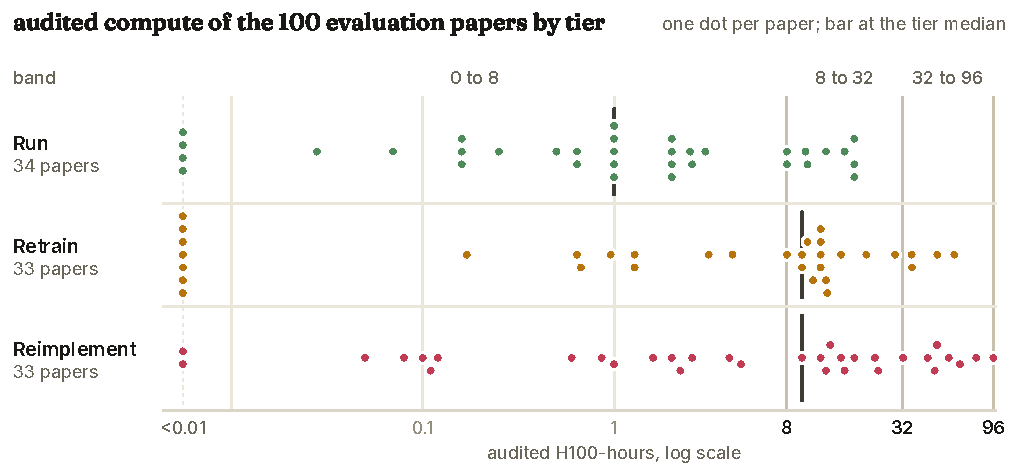
\includegraphics[width=\textwidth]{figures/app_EF_compute_strip}
\caption{The audited compute of the 100 evaluation papers, one dot per paper
on a log axis, with a bar at each tier's median and papers below the axis
floor in the leftmost slot.}
\label{fig:app-ef-compute-strip}
\end{figure}

\begin{figure}[htb]
\centering
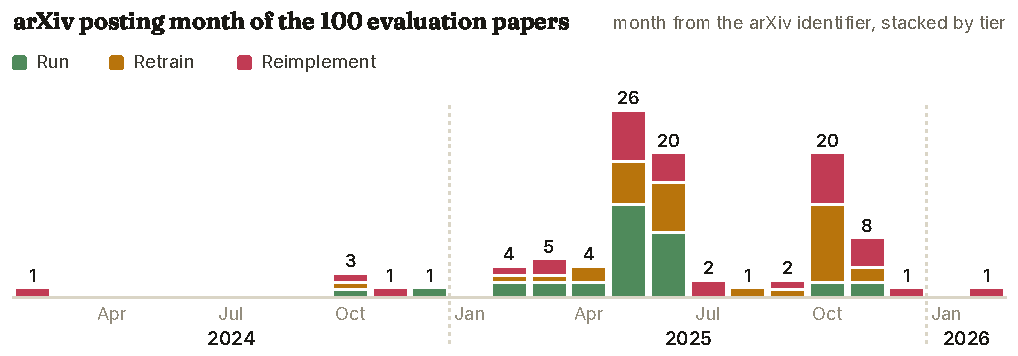
\includegraphics[width=\textwidth]{figures/app_EF_arxiv_months}
\caption{The 100 evaluation papers by the month of their arXiv identifier,
stacked by tier.}
\label{fig:app-ef-arxiv-months}
\end{figure}
